\subsubsection*{Classification of Quadric Surface in $\mathbb{R}^3$}

\begin{enumerate}
    \item $\operatorname{rank}A=3$

          $(+,+,+;+)\quad \frac{x^2}{a^2}+\frac{y^2}{b^2}+\frac{z^2}{c^2}=1$ \raisebox{-0.5\height}{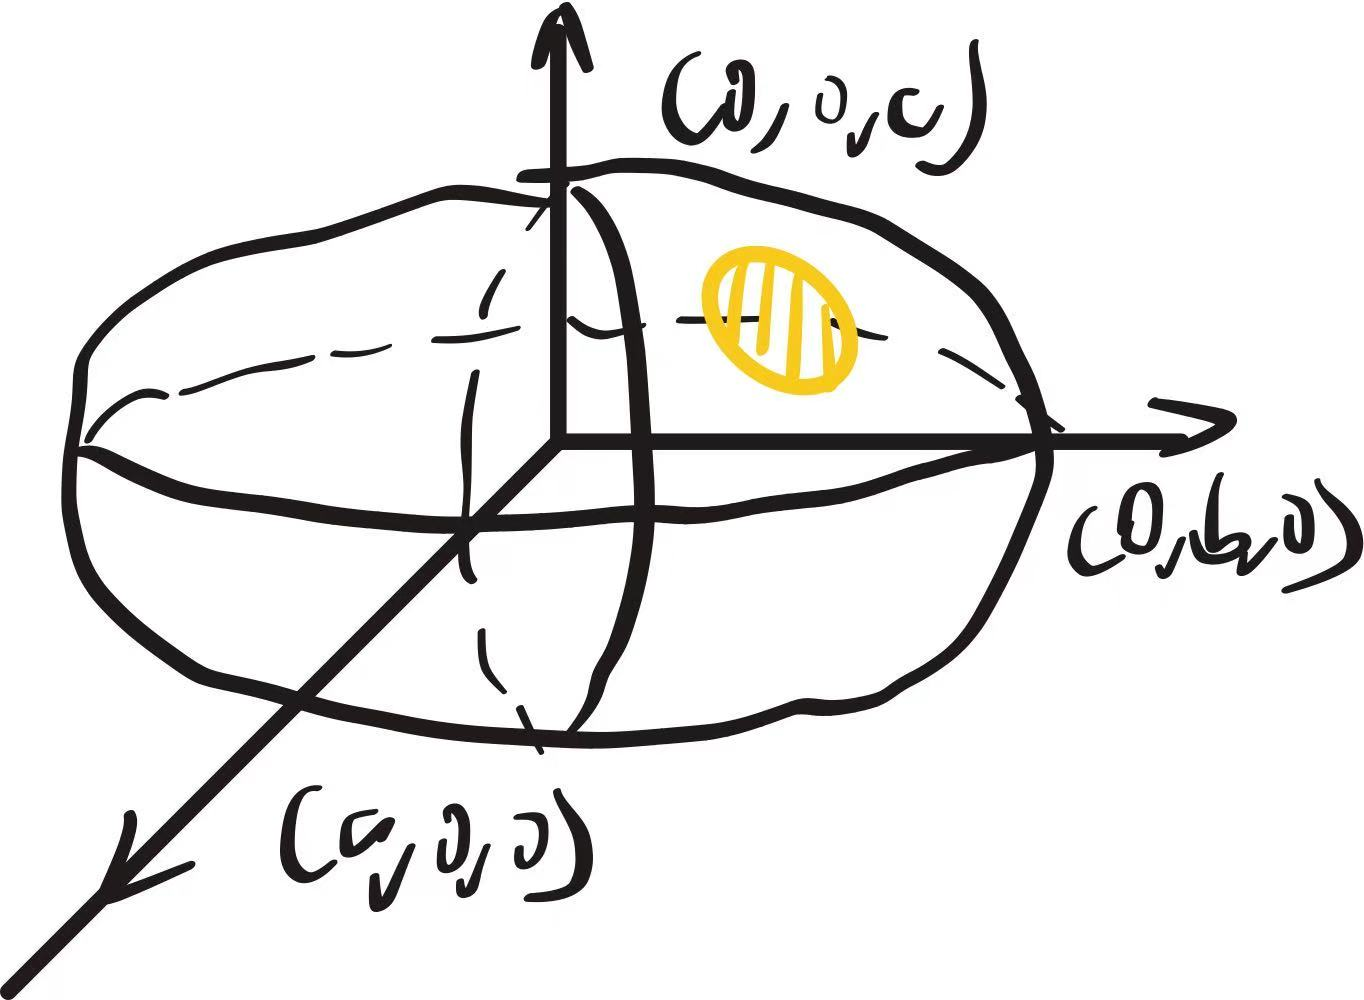
\includegraphics[height=3cm]{chapters/08/ellipsoid}} ellipsoid

          $(+,+,+;0)\quad \frac{x^2}{a^2}+\frac{y^2}{b^2}+\frac{z^2}{c^2}=0$

          $(+,+,+;-)\quad \frac{x^2}{a^2}+\frac{y^2}{b^2}+\frac{z^2}{c^2}=-1$

          $(+,+,-;+)\quad \frac{x^2}{a^2}+\frac{y^2}{b^2}-\frac{z^2}{c^2}=1$ \raisebox{-0.5\height}{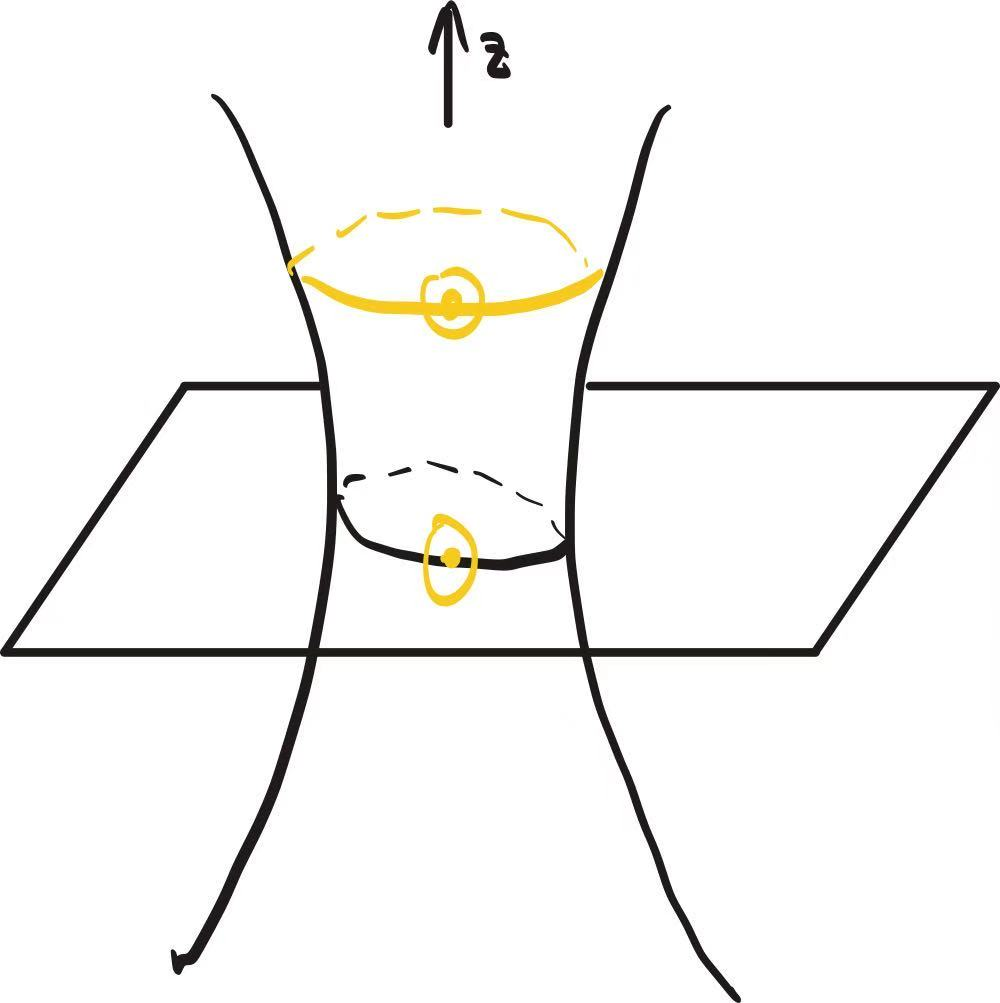
\includegraphics[height=3cm]{chapters/08/sshyperboloid}} single sheeted hyperboloid 单叶双曲面

          $(+,+,-;0)\quad \frac{x^2}{a^2}+\frac{y^2}{b^2}-\frac{z^2}{c^2}=0$ \raisebox{-0.5\height}{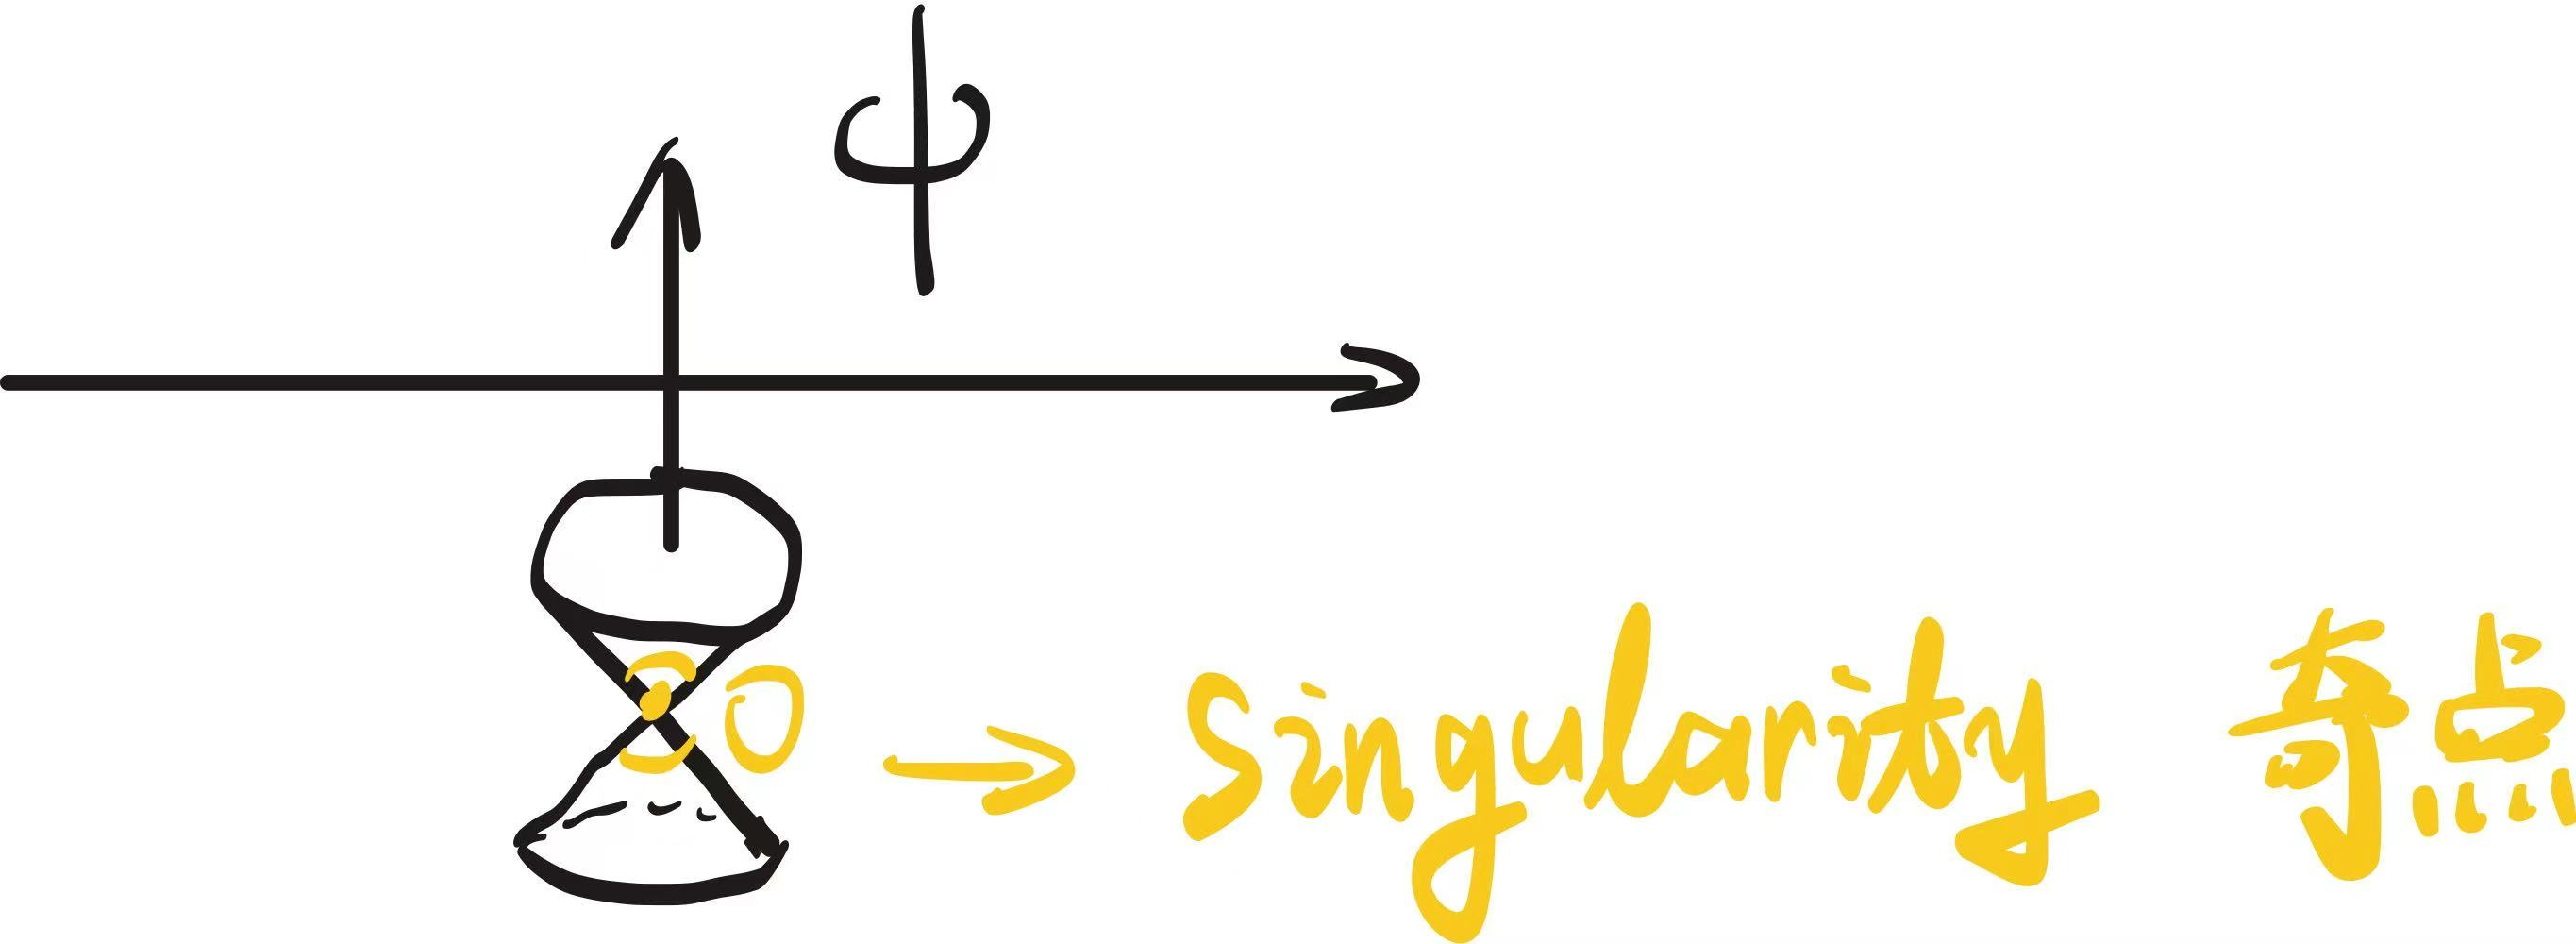
\includegraphics[height=2cm]{chapters/08/sing}}

          $(+,+,-;-)\quad \frac{x^2}{a^2}+\frac{y^2}{b^2}-\frac{z^2}{c^2}=-1$ \raisebox{-0.5\height}{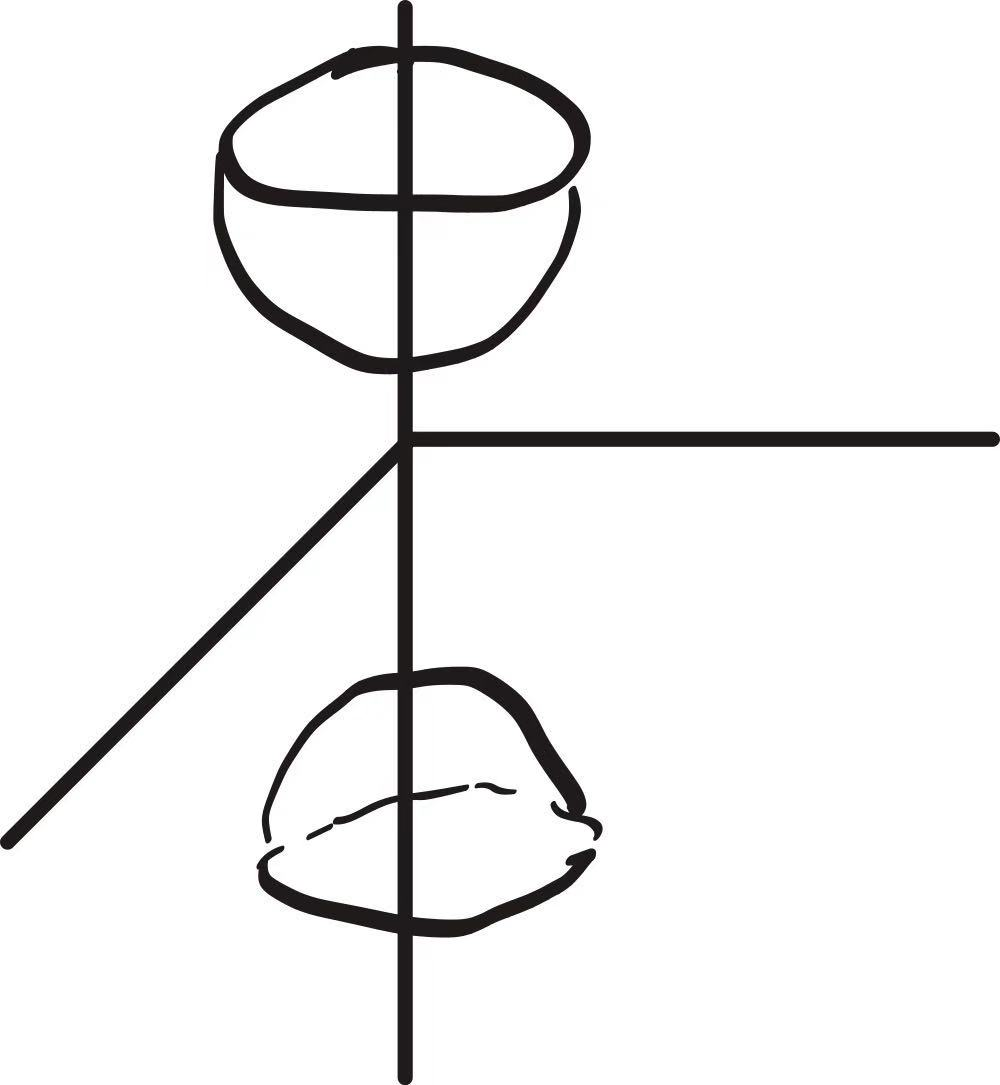
\includegraphics[height=3cm]{chapters/08/dshyperboloid}} Double sheeted hyperboloid 双叶双曲面
    \item $\operatorname{rank}A=2$

          $(+,+,0;+;0)\quad\frac{x^2}{a^2}+\frac{y^2}{b^2}+z=0$ \raisebox{-0.5\height}{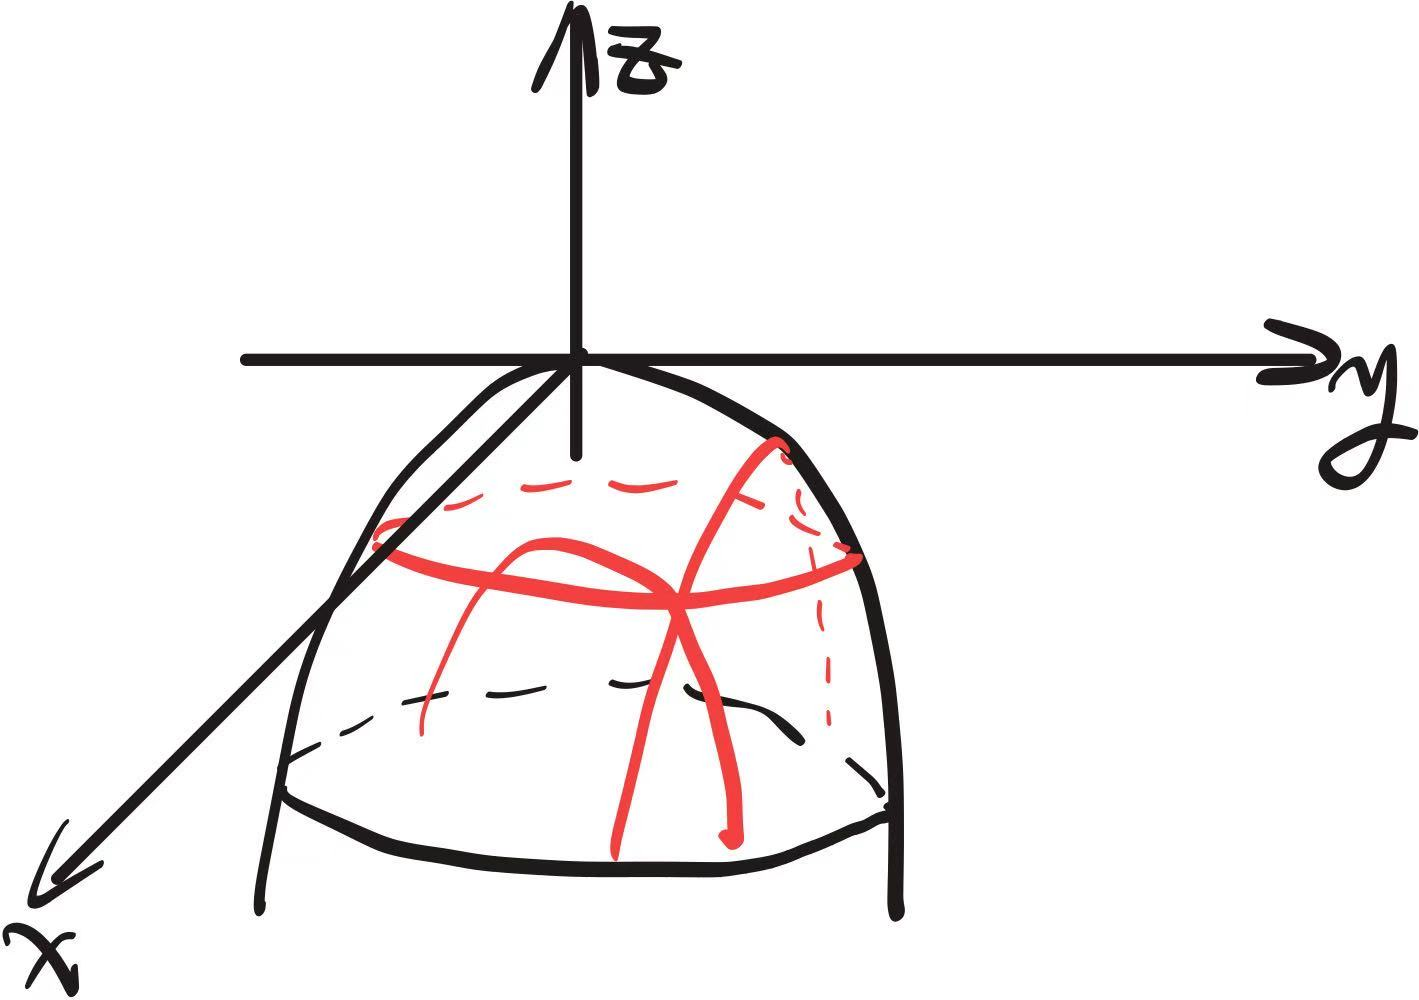
\includegraphics[height=3cm]{chapters/08/elpa}} Elliptical paraboloid 椭圆抛物面

          $(+,+,0;0;+)\quad\frac{x^2}{a^2}+\frac{y^2}{b^2}=1$ \raisebox{-0.5\height}{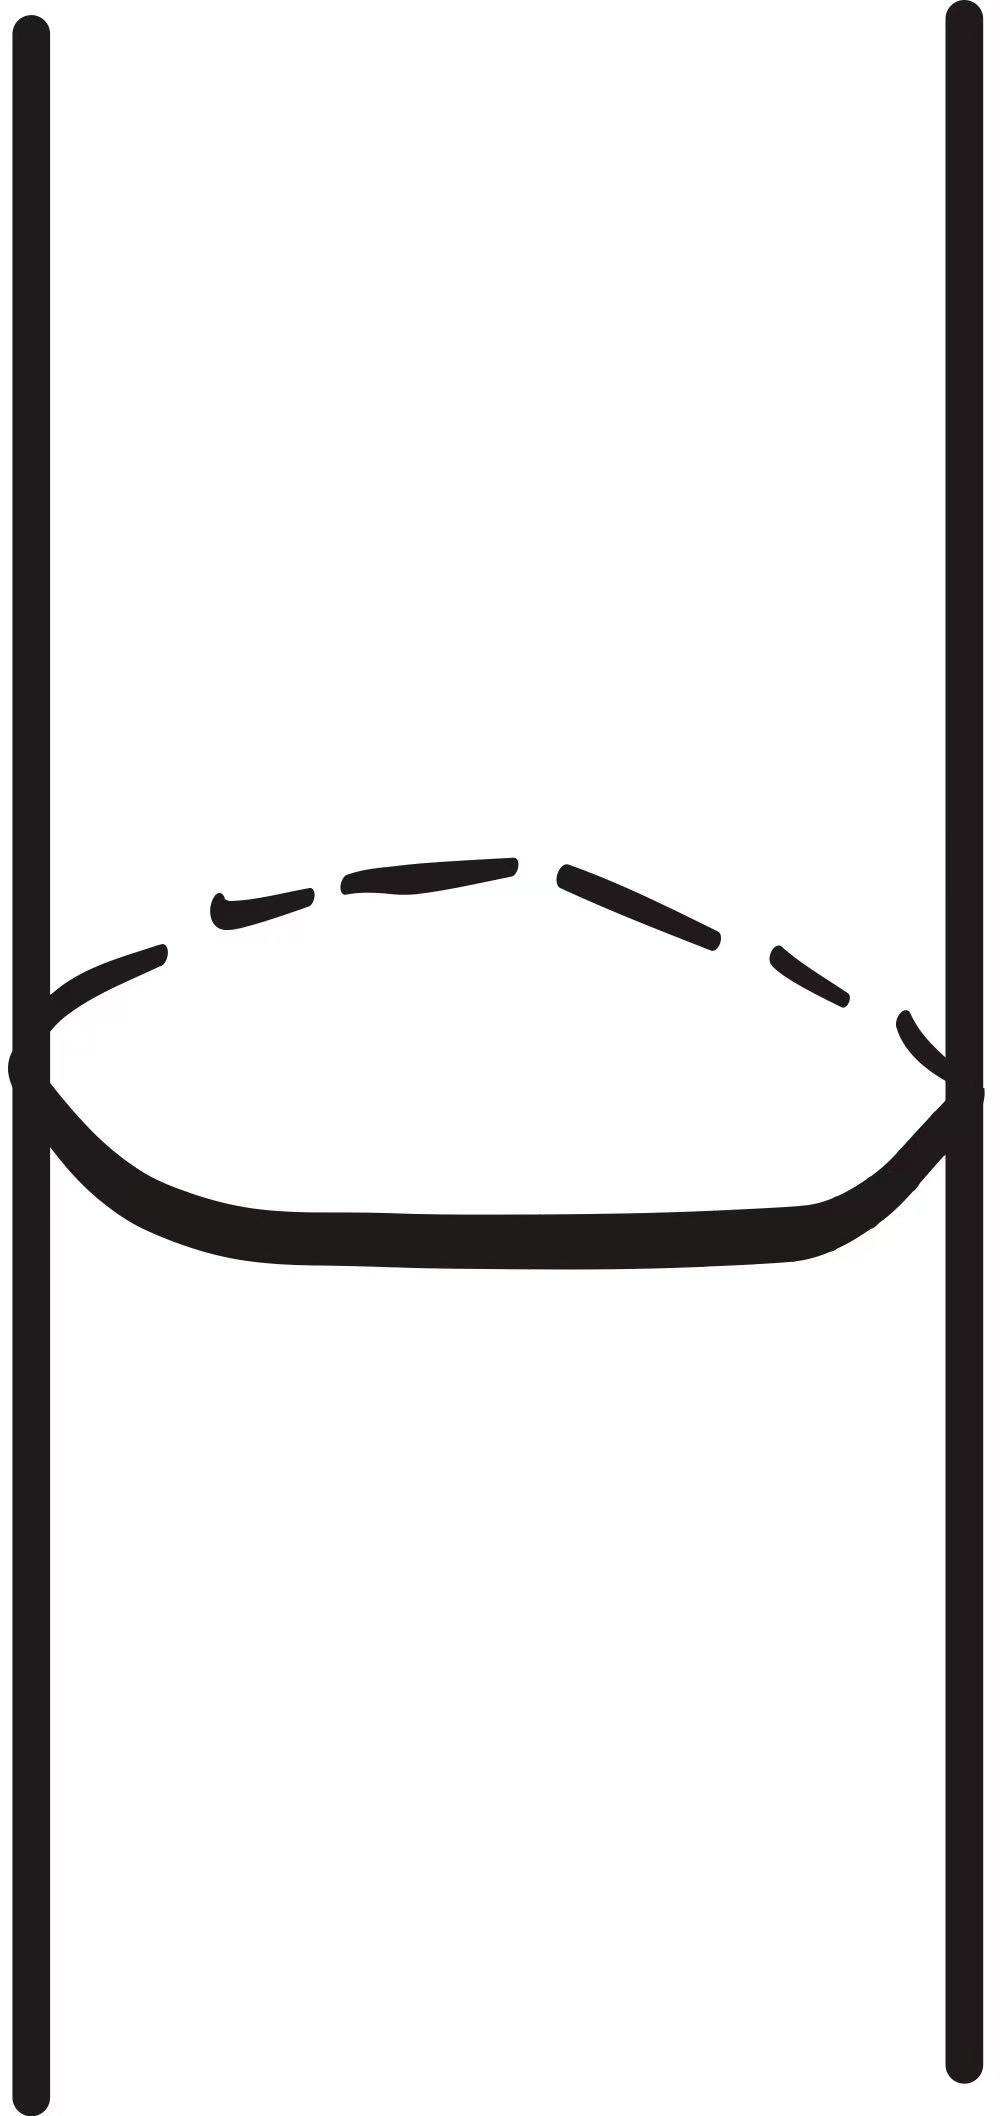
\includegraphics[height=2cm]{chapters/08/elcy}} Elliptical cylinder 椭圆柱面

          $(+,-,0;+;0)\quad\frac{x^2}{a^2}-\frac{y^2}{b^2}+z=0$ \raisebox{-0.5\height}{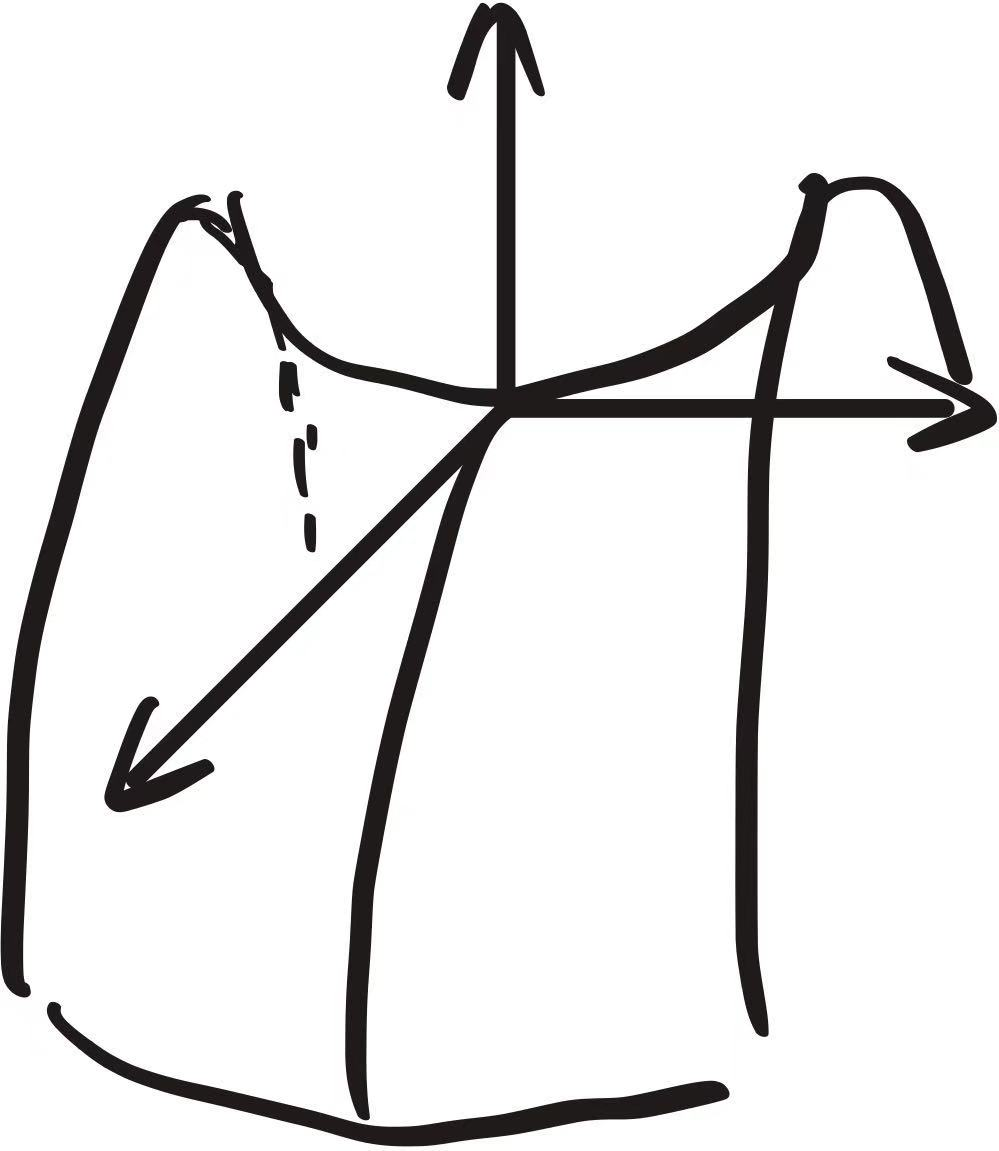
\includegraphics[height=3cm]{chapters/08/hypa}} $\substack{\text{Hyperbolical paraboloid/}\\\text{Saddle surface}}$ 鞍面

          $\begin{cases}
                  (+,-,0;0;+)\quad\frac{x^2}{a^2}-\frac{y^2}{b^2}=1 \\
                  (+,-,0;0;-)\quad\frac{x^2}{a^2}-\frac{y^2}{b^2}=-1
              \end{cases}$ \raisebox{-0.5\height}{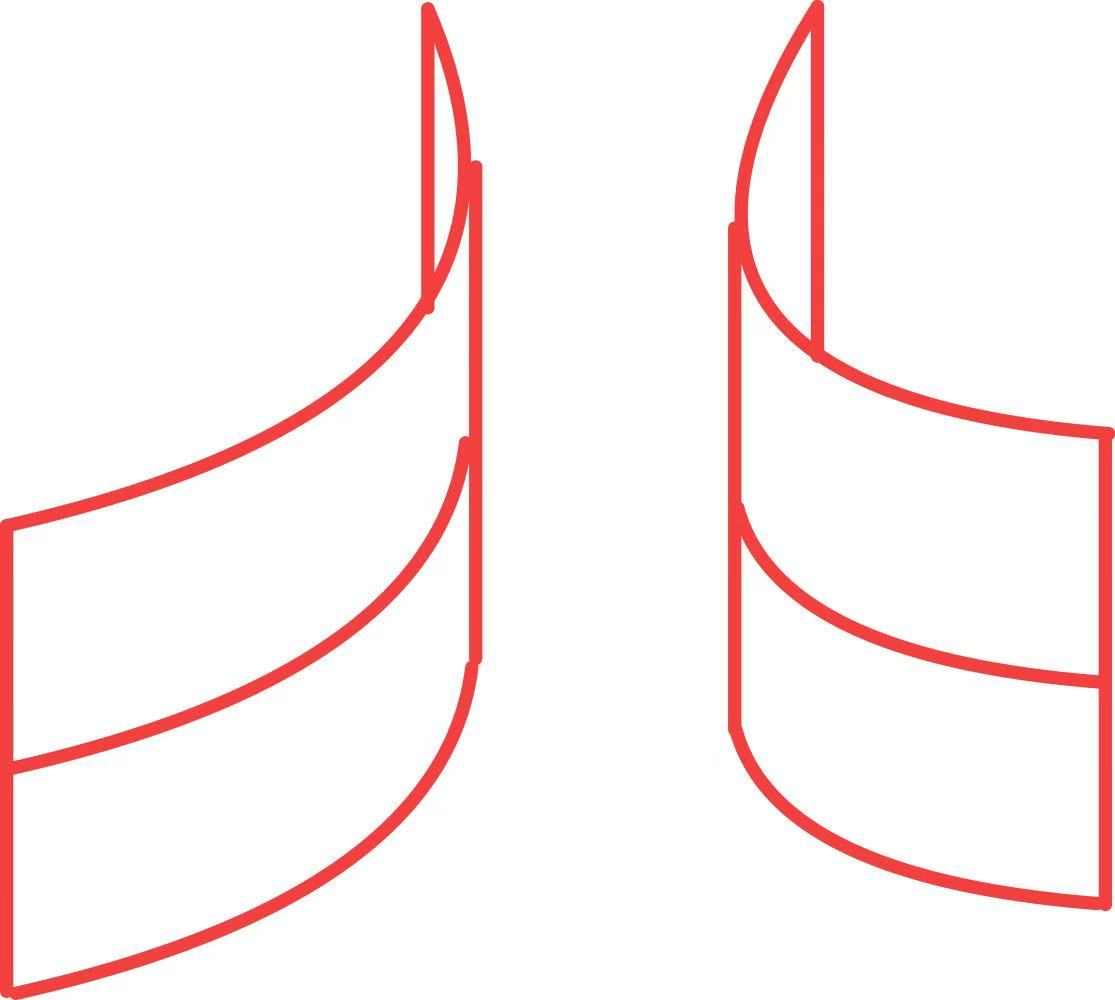
\includegraphics[height=3cm]{chapters/08/hycy}} Hyperbolical cylinder

          $(+,-,0;-;0)\quad\frac{x^2}{a^2}-\frac{y^2}{b^2}=0$ \raisebox{-0.5\height}{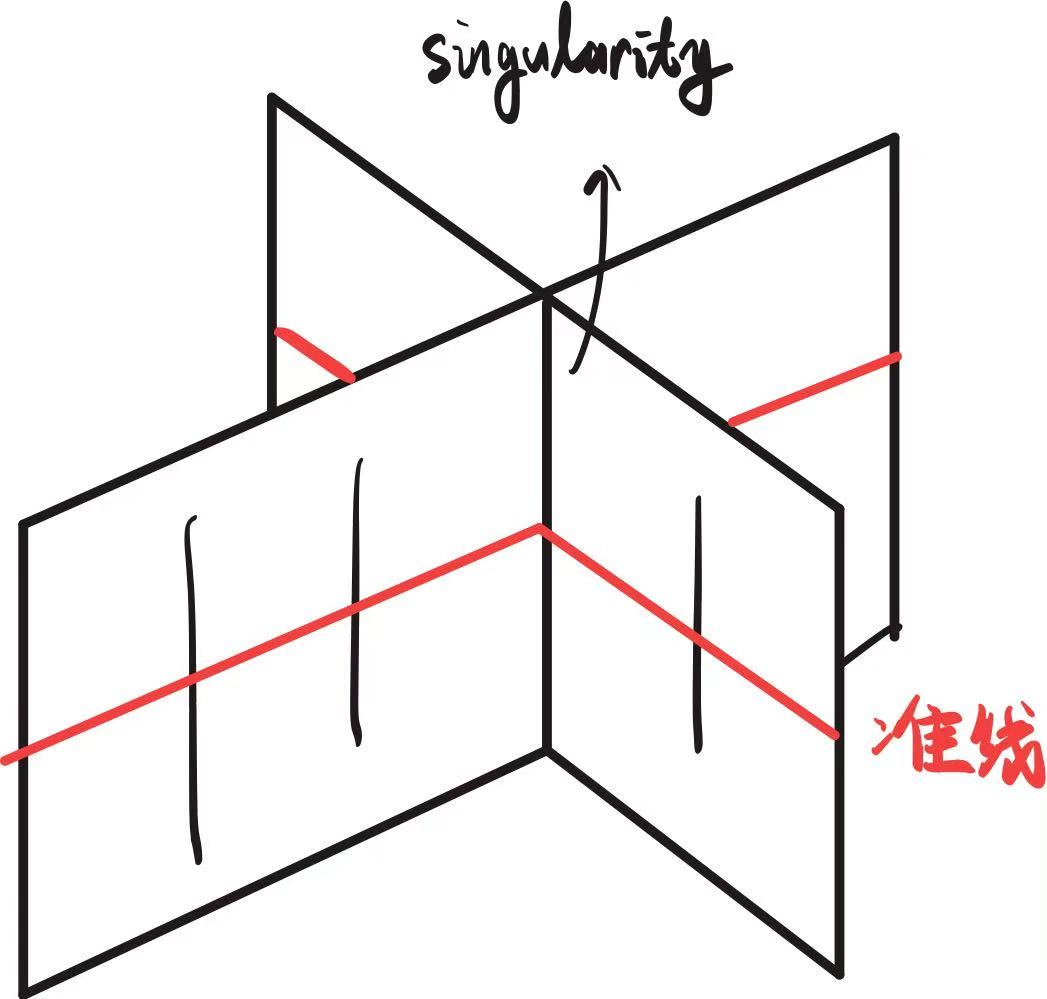
\includegraphics[height=3cm]{chapters/08/twoplanex}}
    \item $\operatorname{rank}A=1$

          $(+,0,0;+;0)\quad\frac{x^2}{a^2}+y=0$ \raisebox{-0.5\height}{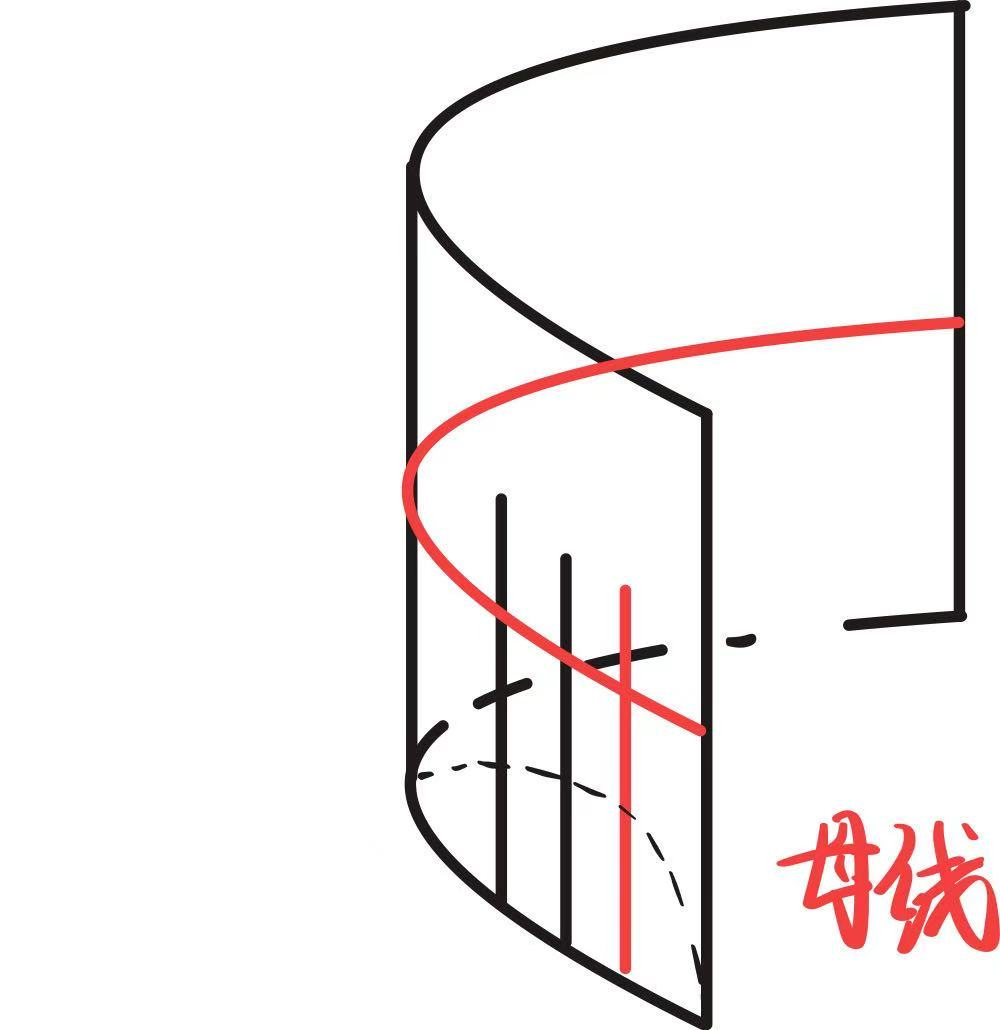
\includegraphics[height=3cm]{chapters/08/shycy}}

          $(+,0,0;0;+)$ \raisebox{-0.5\height}{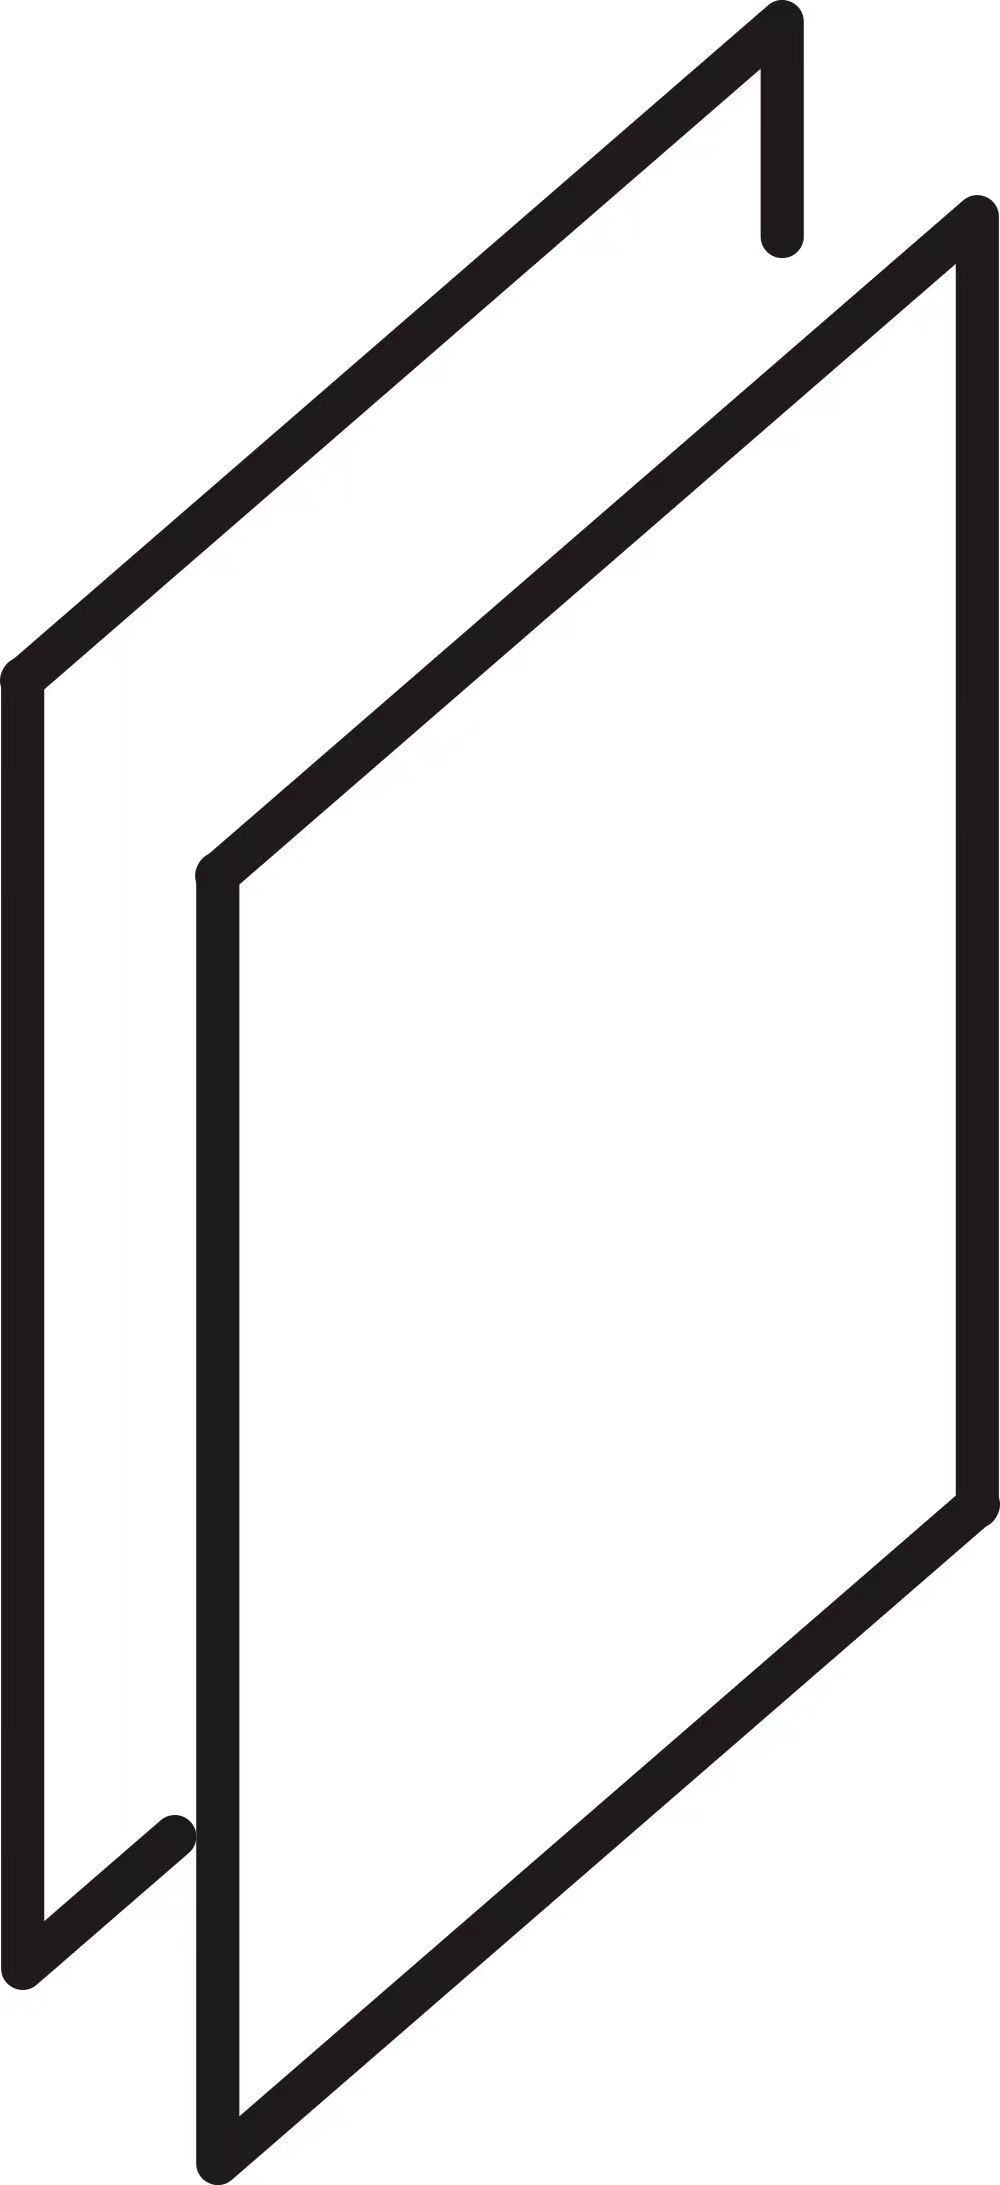
\includegraphics[height=3cm]{chapters/08/twoplanep}} Double plane

          $(+,0,0;0;0)$

          $(+,0,0;0;-)\rightarrow\emptyset$
\end{enumerate}

\subsubsection*{Intersection of Quadric Surface and Plane}

$$\begin{cases}
        f\left(\overrightarrow{x}\right)=\overrightarrow{x}^TA\overrightarrow{x}+\overrightarrow{b}^T\overrightarrow{x}+c=0 \\
        \overrightarrow{n}^T\overrightarrow{x}+d=0
    \end{cases}\quad\begin{cases}
        x^2+y^2+z^2=1 \\
        (x-a)^2+y^2=r^2
    \end{cases}\raisebox{-0.5\height}{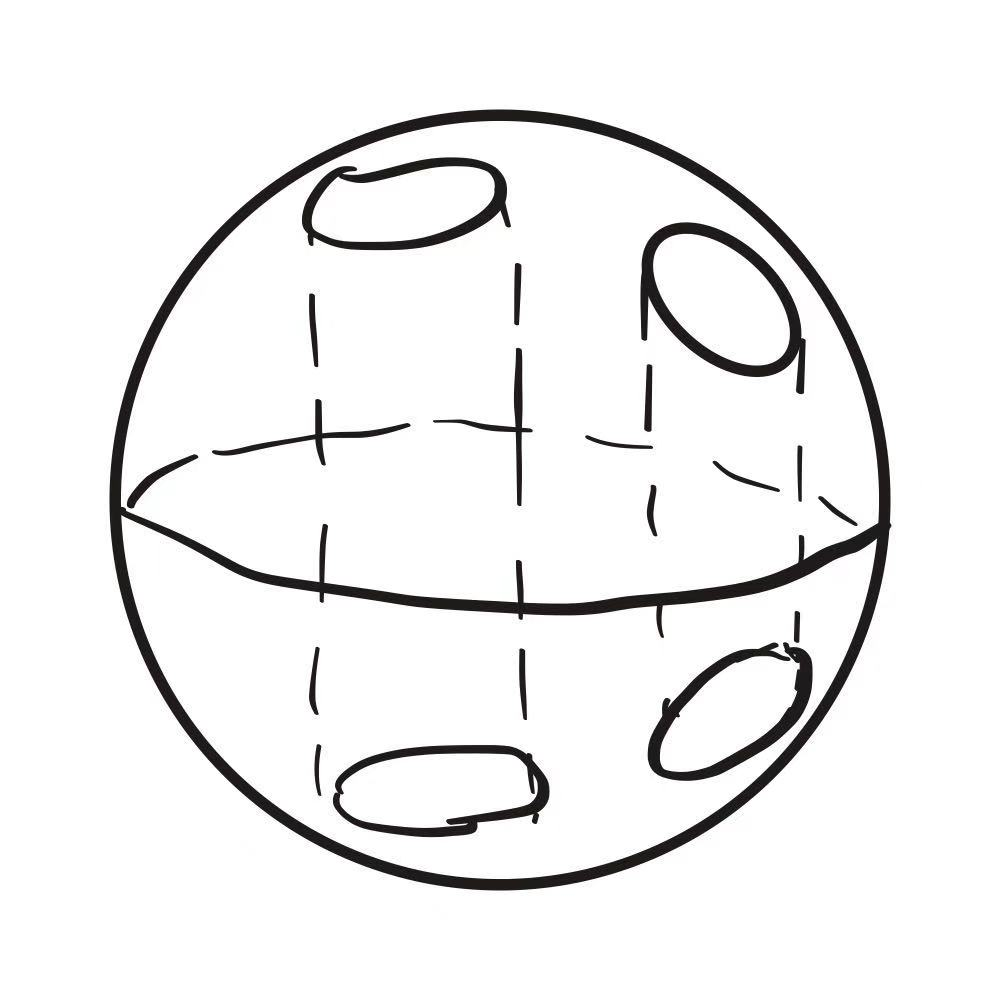
\includegraphics[height=3cm]{chapters/08/intersection}}$$

\subsubsection*{Surface of Revolution 旋转}

\raisebox{-0.5\height}{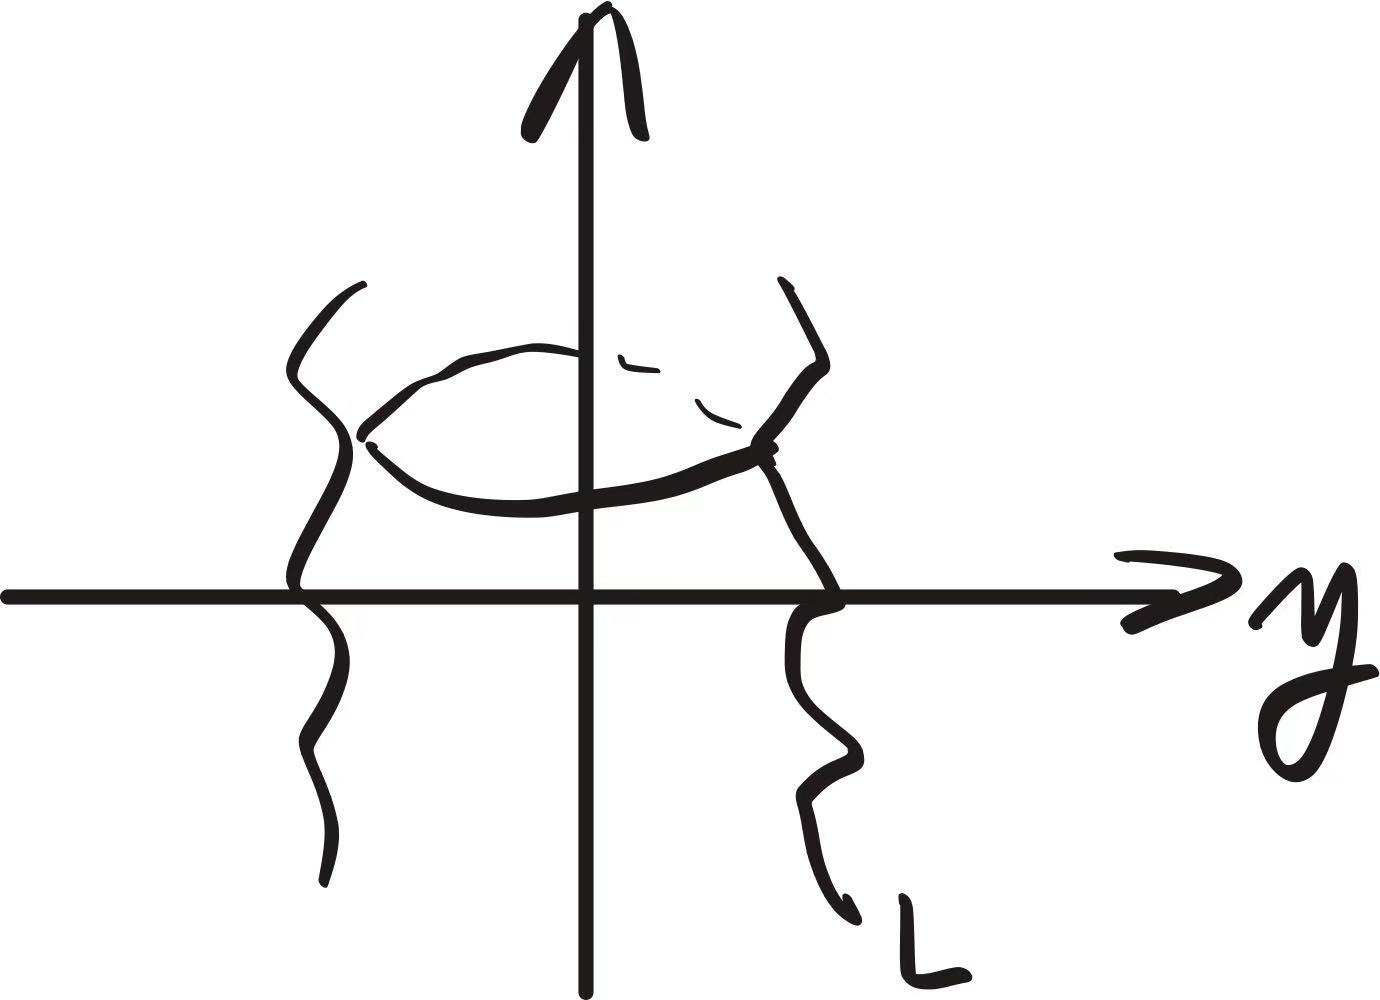
\includegraphics[height=3cm]{chapters/08/sor1}}

$F(y,z)=0\rightarrow$ curve $L$ revolved along $Z$ axis $\implies$ Surface implicit equation?

\begin{align*}
    \raisebox{-0.5\height}{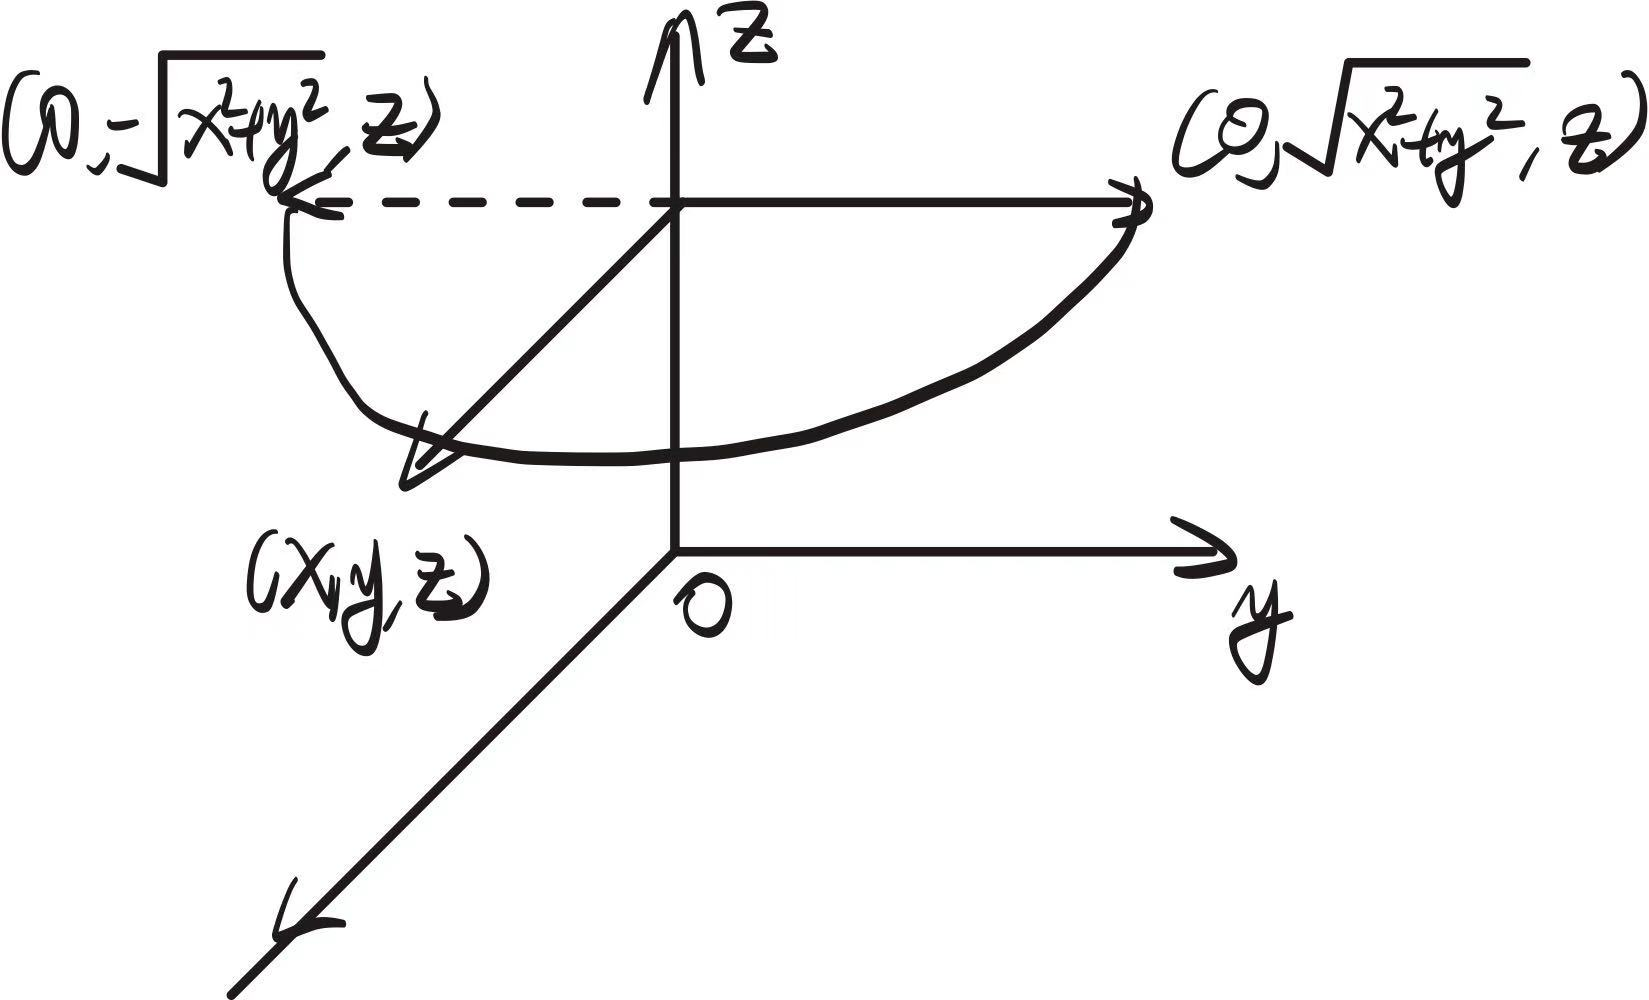
\includegraphics[height=3cm]{chapters/08/sor2}} & \implies F\left(\pm\sqrt{x^2+y^2},z\right)=0          \\
                                                                           & \iff (x,y,z)\text{ lies on the surface of revolution}
\end{align*}

\begin{example}
    \raisebox{-1\height}{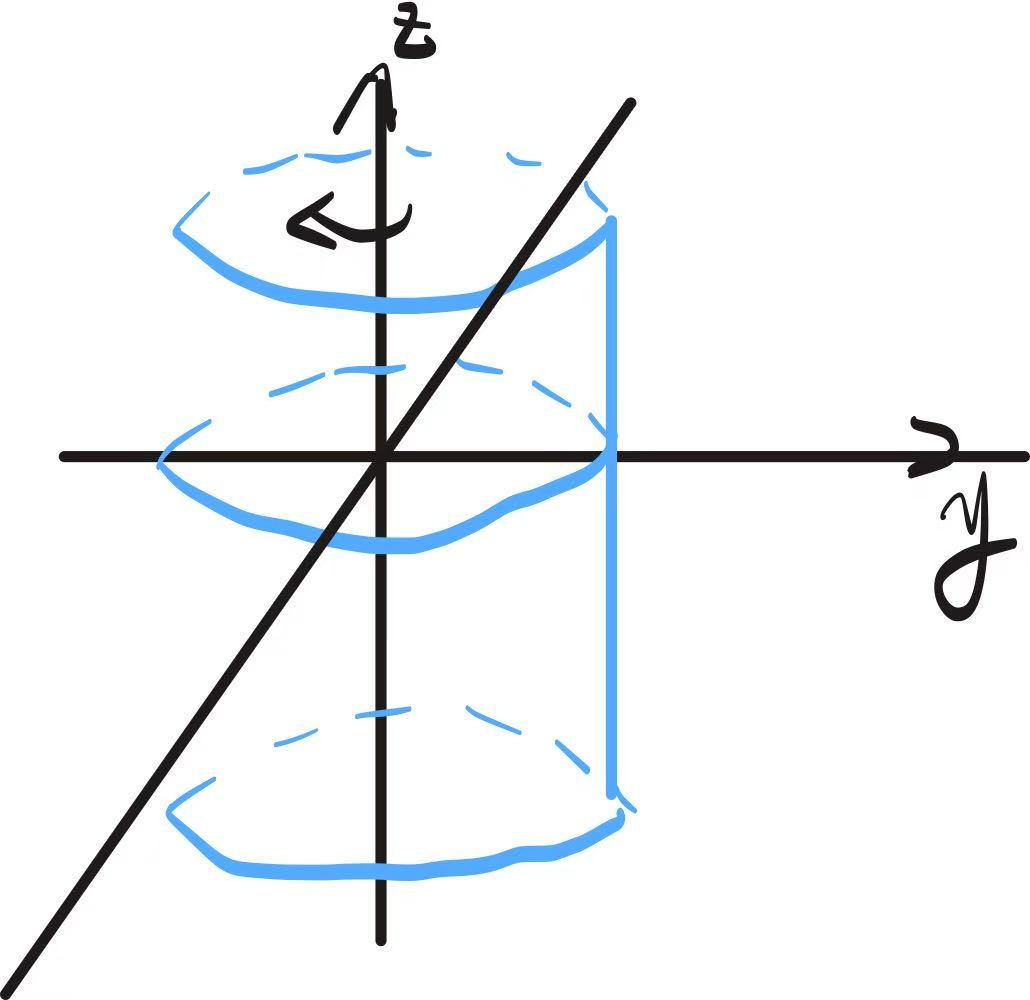
\includegraphics[height=3cm]{chapters/08/sor3}} $L=\left\{(0,y,z)\mid y=z\right\}$

    \raisebox{-0.5\height}{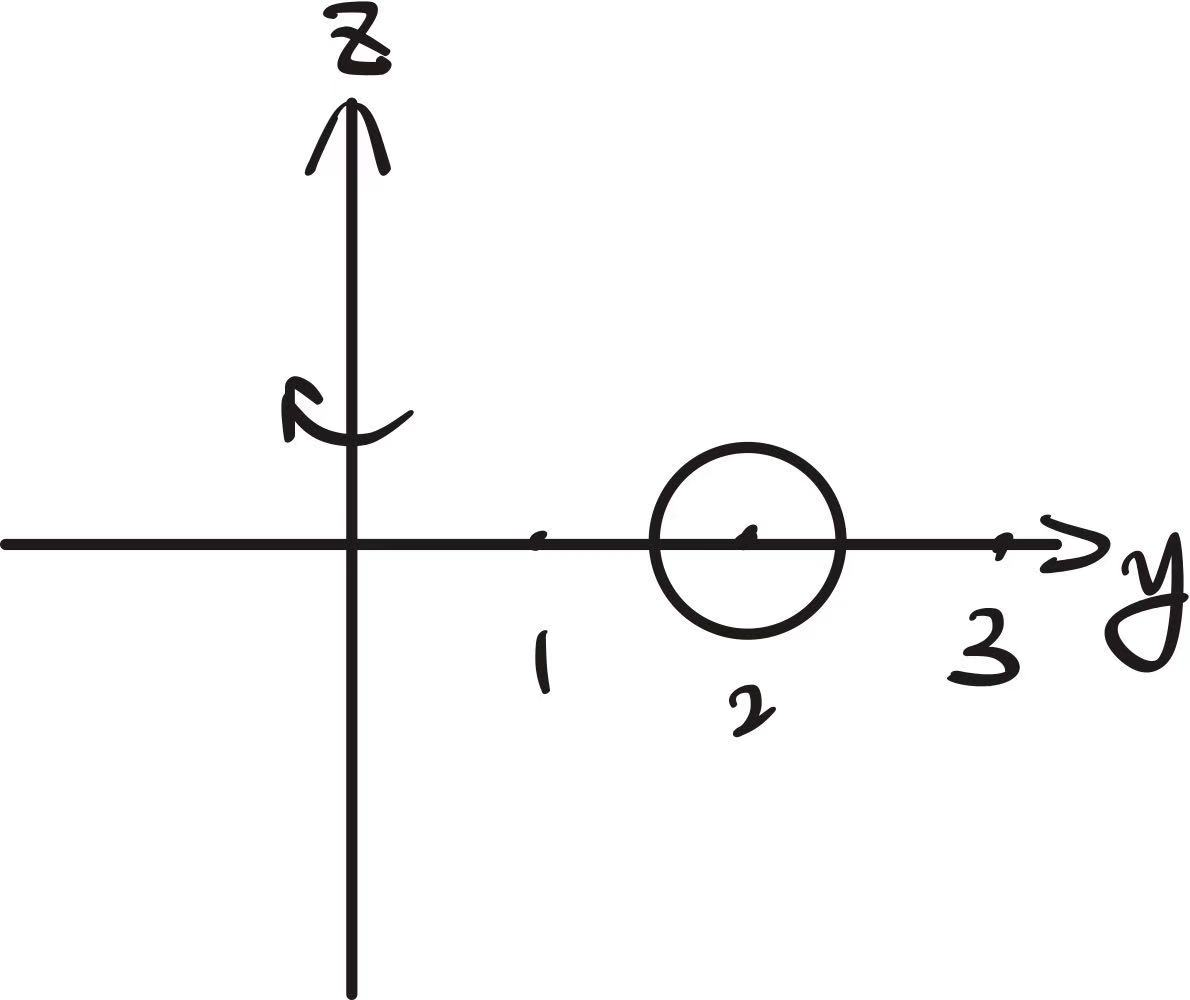
\includegraphics[height=3cm]{chapters/08/sor4}} $\substack{\pm\sqrt{x^2+y^2}=z\leftrightsquigarrow x^2+y^2-z^2=0\quad\\
            x^2+y^2+4\pm 4\sqrt{x^2+y^2}+z^2=1\implies\left(x^2+y^2+z^2+3\right)^2=16\left(x^2+y^2\right)\\
            (y-2)^2+z^2=1\leadsto \left(\pm\sqrt{x^2+y^2}-2\right)^2+z^2=1}$
\end{example}